\documentclass[../main.tex]{subfiles}
\begin{document}
\subsection{Coordinate polari}
\begin{itemize}
    \item Coordinate cartesiane, $P=(x,y)$ (ascissa, ordinata)
    \item Coordinate polari, $P=(r,\alpha)$ (norma, angolo)
\end{itemize}
\vspace{1cm}

Per passare da coordinate polari a coordinate cartesiane si utilizzano rispettivamente $cos(\alpha)$ e $sin(\alpha)$. Vale dunque:
$$
    \begin{cases}
        x = r\phantom{.}cos(\alpha) \\
        y = r\phantom{.}sin(\alpha)
    \end{cases}
$$
che graficamente appare:
\begin{figure}[h]
    \centering
    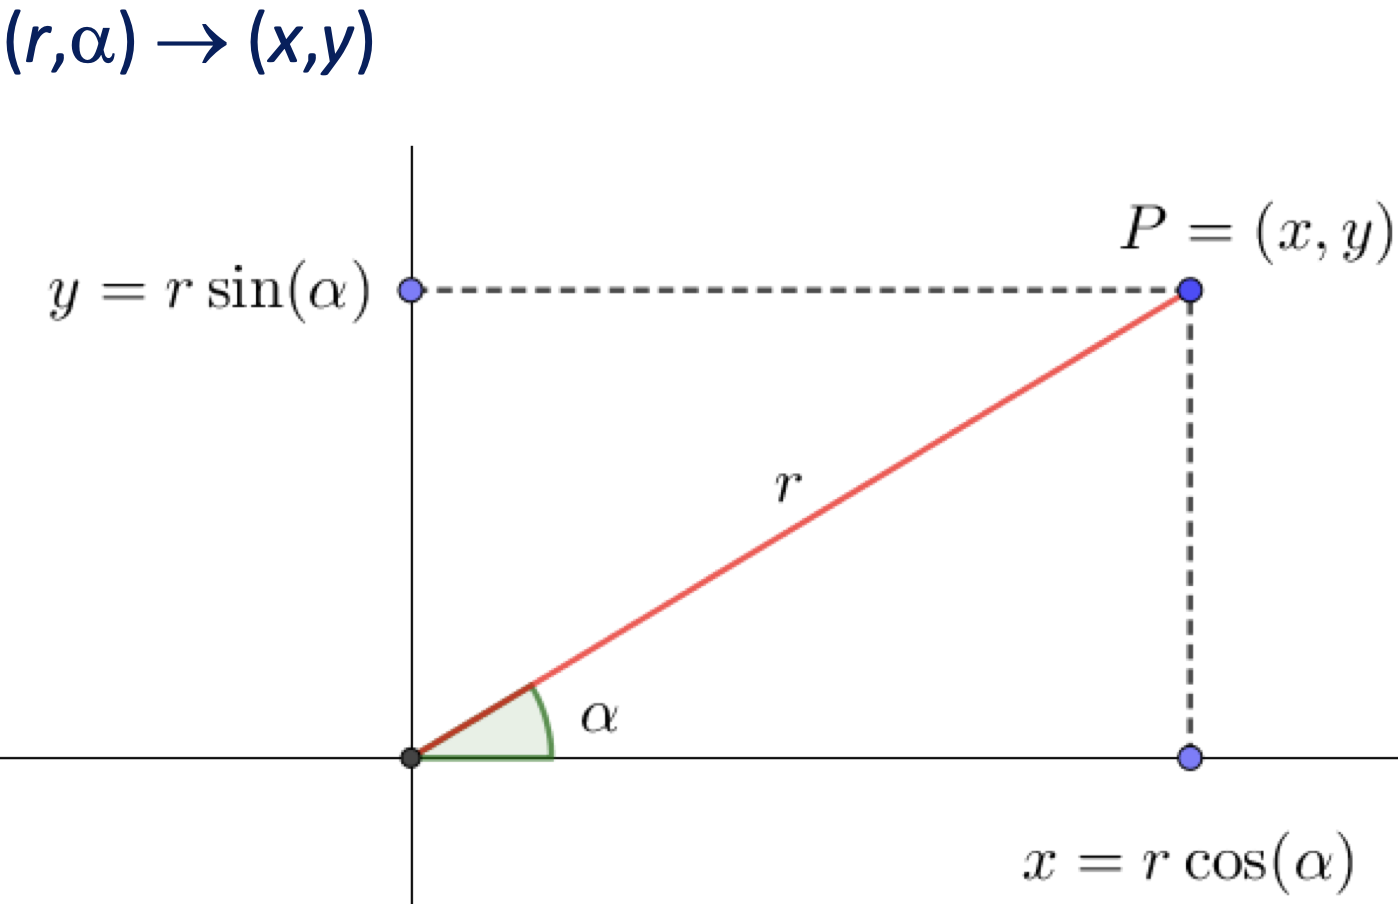
\includegraphics[width=0.6\textwidth]{../images/polariCartesiane.png}
\end{figure}

\vspace{2cm}
Per passare invece da coordinate cartesiane a coordinate polari dobbiamo stabilire $r$ e $\alpha$. Abbiiamo quindi:
$$
    \begin{cases}
        r = \sqrt{x^2 + y^2} \\
        \alpha = \begin{cases}
            cos^{-1}(\frac{x}{r}) \phantom{--} y \geq 0 \\
            -cos^{-1}(\frac{x}{r}) \phantom{-} y < 0
        \end{cases}
    \end{cases}
$$
che graficamente appare:
\begin{figure}[h]
    \centering
    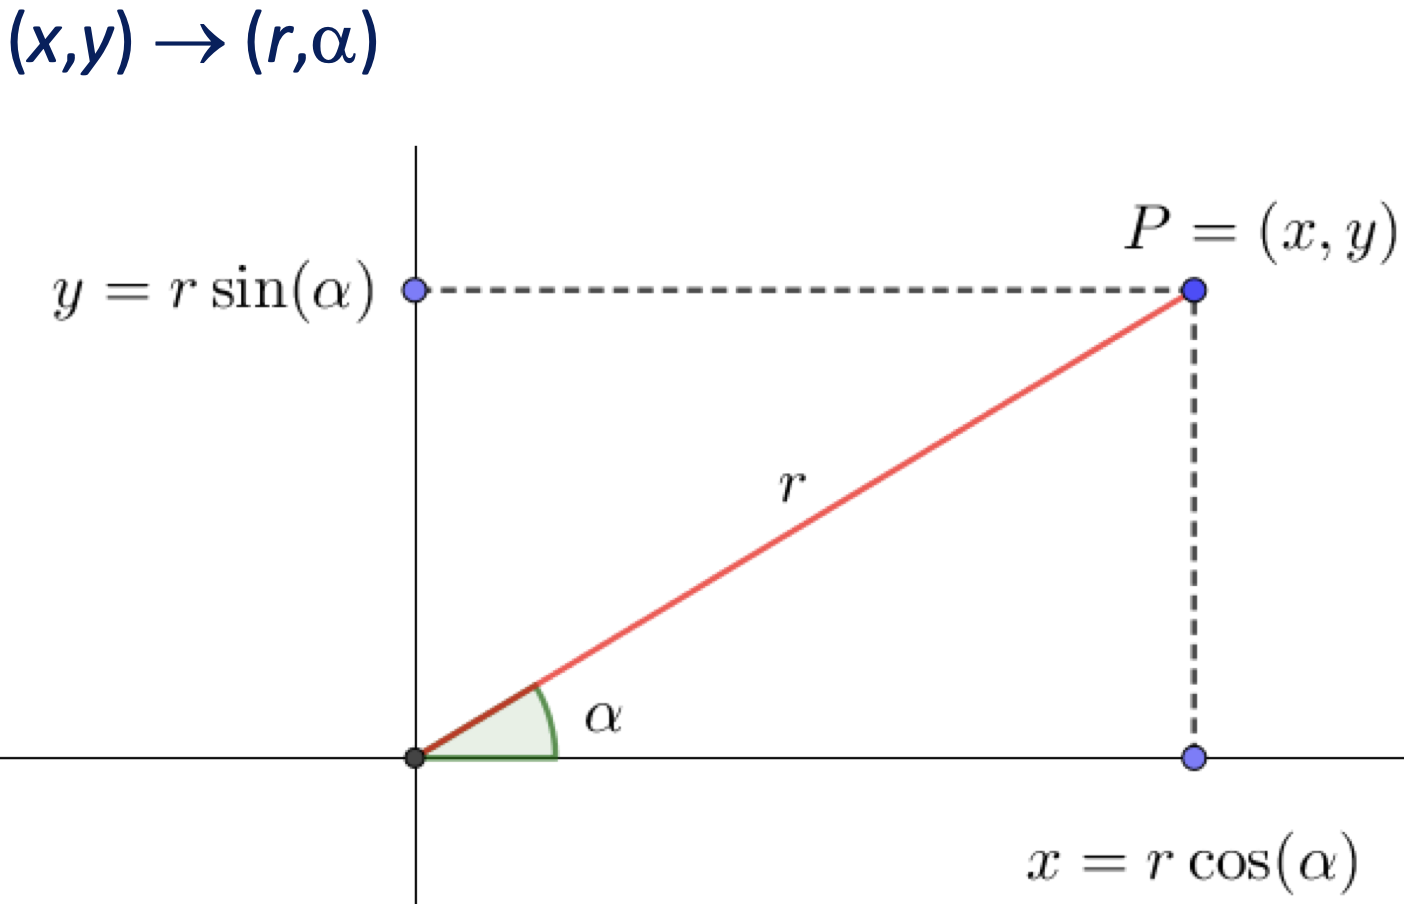
\includegraphics[width=0.6\textwidth]{../images/cartesianePolari.png}
\end{figure}

\subsection{Il prodotto scalare}
\subsubsection{norma}
Dato il vettore $x$ si chiama prodotto scalare di $x$ per se stesso e si indica $x \cdot x$ il numero reale
$$
   \mathbb{R}^2 \text{: } x \cdot x = \begin{pmatrix} x_1 \\ x_2 \end{pmatrix} \cdot \begin{pmatrix} x_1 \\ x_2 \end{pmatrix} 
   = x^2_1 + x^2_2 = \left\lVert x \right\rVert^2
$$
dunque la norma è
$$
    \left\lVert x \right\rVert = \sqrt{x \cdot x}
$$
questo vale in qualsiasi dimensione ($\mathbb{R}^n$).

\vspace{0.5cm}
La norma è un valore sempre maggiore o, nel caso il vettore fosse nullo, uguale a zero. Inoltre possiede due proprietà interessanti:
\begin{itemize}
    \item \textbf{disuguaglianza triangolare}, $\left\lVert x + y \right\rVert \leq \left\lVert x \right\rVert + \left\lVert x \right\rVert$
    \item \textbf{omogeneità}, $\left\lVert hx \right\rVert = \left\lvert h \right\rvert + \left\lVert x \right\rVert $
\end{itemize}
La somma di due norme non è quindi uguale alla norma contenente la somma dei due vettori (disuguaglianza triangolare).

\vspace{1.5cm}
\subsubsection{I versori}
I versori sono vettori di norma $1$, per fare diventare un vettore generico $\left\lVert x \right\rVert$ di norma $1$ si può fare
$$
    \frac{1}{\left\lVert x \right\rVert } x  \phantom{--}\text{ questo vettore ha norma 1}
$$

Allo stesso modo se vogliamo farlo diventare, per esempio, di norma $7$ possiamo scriverlo come
$$
    \frac{7}{\left\lVert x \right\rVert } x \phantom{--} \text{ questo vettore ha norma 7}
$$

\vspace{1.5cm}
\subsubsection{Prodotto scalare x$\cdot$y}
Dati i vettori $x = \begin{pmatrix}x_1 \\ x_2 \\ ... \\ x_n \end{pmatrix}, y = \begin{pmatrix}y_1 \\ y_2 \\ ... \\ y_n \end{pmatrix} \in \mathbb{R}^n$,
si chiama prodotto scalare di $x$ e $y$, e si indica $x \cdot y$, il numero reale
$$
    x \cdot y = x_1y_1 + x_2y_2 + ... + x_ny_n
$$

Di base se prendiamo due vettori tramite l'agolo che generano possiamo determinare:
\begin{itemize}
    \item se $\alpha > 90^{\circ}$ il prodotto scalare è negativo
    \item se $\alpha = 90^{\circ}$ il prodotto scalare è $0$
    \item se $\alpha < 90^{\circ}$ il prodotto scalare è positivo
\end{itemize}

\vspace{1cm}
\subsubsection{Teorema del prodotto scalare}
$$
   u \cdot v = \left\lVert u \right\rVert \left\lVert v \right\rVert cos(\alpha)
$$
dalla quale possiamo ricavare
$$
    cos(\alpha) = \frac{u \cdot v}{\left\lVert u\right\rVert \left\lVert v\right\rVert }
$$
e quindi
$$
    \alpha = cos^{-1}\left( \frac{u \cdot v}{\left\lVert u \right\rVert \left\lVert v \right\rVert } \right)
$$
\textbf{Nota:} $\alpha rad = \frac{\pi}{180} \alpha^\circ $

\vspace{0.5cm}
\subsubsection{Applicazioni}
\begin{itemize}
    \item \textbf{Vettore bisecante:} Dati due vettori $\vec{a}$ e $\vec{b}$ si vuole costruire un vettore $\vec{c}$ che divide l'angolo
    tra $\vec{a}$ e $\vec{b}$ in due angoli uguali:
    \begin{center}
        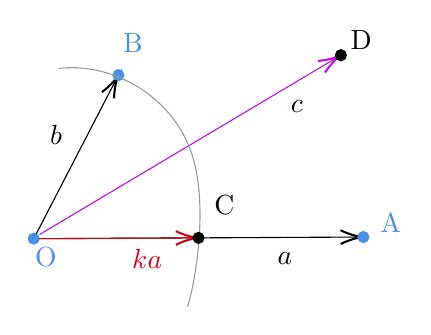
\begin{tikzpicture}[x=0.75pt,y=0.75pt,yscale=-1,xscale=1]
            %Straight Lines [id:da8999915472425152] 
            \draw    (210.6,130.6) -- (250.48,53.58) ;
            \draw [shift={(251.4,51.8)}, rotate = 117.37] [color={rgb, 255:red, 0; green, 0; blue, 0 }  ][line width=0.75]    (10.93,-3.29) .. controls (6.95,-1.4) and (3.31,-0.3) .. (0,0) .. controls (3.31,0.3) and (6.95,1.4) .. (10.93,3.29)   ;
            %Straight Lines [id:da7612845637763869] 
            \draw    (210.6,130.6) -- (367.4,129.81) ;
            \draw [shift={(369.4,129.8)}, rotate = 179.71] [color={rgb, 255:red, 0; green, 0; blue, 0 }  ][line width=0.75]    (10.93,-3.29) .. controls (6.95,-1.4) and (3.31,-0.3) .. (0,0) .. controls (3.31,0.3) and (6.95,1.4) .. (10.93,3.29)   ;
            %Shape: Circle [id:dp558517833883608] 
            \draw  [color={rgb, 255:red, 74; green, 144; blue, 226 }  ,draw opacity=1 ][fill={rgb, 255:red, 74; green, 144; blue, 226 }  ,fill opacity=1 ] (248.75,51.8) .. controls (248.75,50.34) and (249.94,49.15) .. (251.4,49.15) .. controls (252.86,49.15) and (254.05,50.34) .. (254.05,51.8) .. controls (254.05,53.26) and (252.86,54.45) .. (251.4,54.45) .. controls (249.94,54.45) and (248.75,53.26) .. (248.75,51.8) -- cycle ;
            %Shape: Circle [id:dp4896208528033976] 
            \draw  [color={rgb, 255:red, 74; green, 144; blue, 226 }  ,draw opacity=1 ][fill={rgb, 255:red, 74; green, 144; blue, 226 }  ,fill opacity=1 ] (366.75,129.8) .. controls (366.75,128.34) and (367.94,127.15) .. (369.4,127.15) .. controls (370.86,127.15) and (372.05,128.34) .. (372.05,129.8) .. controls (372.05,131.26) and (370.86,132.45) .. (369.4,132.45) .. controls (367.94,132.45) and (366.75,131.26) .. (366.75,129.8) -- cycle ;
            %Shape: Circle [id:dp29559362996381155] 
            \draw  [color={rgb, 255:red, 74; green, 144; blue, 226 }  ,draw opacity=1 ][fill={rgb, 255:red, 74; green, 144; blue, 226 }  ,fill opacity=1 ] (207.95,130.6) .. controls (207.95,129.14) and (209.14,127.95) .. (210.6,127.95) .. controls (212.06,127.95) and (213.25,129.14) .. (213.25,130.6) .. controls (213.25,132.06) and (212.06,133.25) .. (210.6,133.25) .. controls (209.14,133.25) and (207.95,132.06) .. (207.95,130.6) -- cycle ;
            %Straight Lines [id:da8517893456688485] 
            \draw [color={rgb, 255:red, 189; green, 16; blue, 224 }  ,draw opacity=1 ]   (213.4,128.6) -- (356.88,43.22) ;
            \draw [shift={(358.6,42.2)}, rotate = 149.25] [color={rgb, 255:red, 189; green, 16; blue, 224 }  ,draw opacity=1 ][line width=0.75]    (10.93,-3.29) .. controls (6.95,-1.4) and (3.31,-0.3) .. (0,0) .. controls (3.31,0.3) and (6.95,1.4) .. (10.93,3.29)   ;
            %Shape: Circle [id:dp6964966212295118] 
            \draw  [color={rgb, 255:red, 0; green, 0; blue, 0 }  ,draw opacity=1 ][fill={rgb, 255:red, 0; green, 0; blue, 0 }  ,fill opacity=1 ] (355.95,42.2) .. controls (355.95,40.74) and (357.14,39.55) .. (358.6,39.55) .. controls (360.06,39.55) and (361.25,40.74) .. (361.25,42.2) .. controls (361.25,43.66) and (360.06,44.85) .. (358.6,44.85) .. controls (357.14,44.85) and (355.95,43.66) .. (355.95,42.2) -- cycle ;
            %Straight Lines [id:da11508212585960786] 
            \draw [color={rgb, 255:red, 208; green, 2; blue, 27 }  ,draw opacity=1 ]   (213.25,130.6) -- (288,130.21) ;
            \draw [shift={(290,130.2)}, rotate = 179.7] [color={rgb, 255:red, 208; green, 2; blue, 27 }  ,draw opacity=1 ][line width=0.75]    (10.93,-3.29) .. controls (6.95,-1.4) and (3.31,-0.3) .. (0,0) .. controls (3.31,0.3) and (6.95,1.4) .. (10.93,3.29)   ;
            %Curve Lines [id:da9047542995815328] 
            \draw [color={rgb, 255:red, 155; green, 155; blue, 155 }  ,draw opacity=1 ]   (222.6,48.6) .. controls (247.41,45.47) and (276.36,60.92) .. (286.2,88.2) .. controls (296.04,115.48) and (287.06,157.47) .. (284.6,163.4) ;
            %Shape: Circle [id:dp3889087589538067] 
            \draw  [color={rgb, 255:red, 0; green, 0; blue, 0 }  ,draw opacity=1 ][fill={rgb, 255:red, 0; green, 0; blue, 0 }  ,fill opacity=1 ] (287.35,130.2) .. controls (287.35,128.74) and (288.54,127.55) .. (290,127.55) .. controls (291.46,127.55) and (292.65,128.74) .. (292.65,130.2) .. controls (292.65,131.66) and (291.46,132.85) .. (290,132.85) .. controls (288.54,132.85) and (287.35,131.66) .. (287.35,130.2) -- cycle ;
            
            % Text Node
            \draw (217.2,74.6) node [anchor=north west][inner sep=0.75pt]    {$b$};
            % Text Node
            \draw (326.8,136.2) node [anchor=north west][inner sep=0.75pt]    {$a$};
            % Text Node
            \draw (376.4,117.2) node [anchor=north west][inner sep=0.75pt]   [align=left] {\textcolor[rgb]{0.29,0.56,0.89}{A}};
            % Text Node
            \draw (252.4,30.4) node [anchor=north west][inner sep=0.75pt]   [align=left] {\textcolor[rgb]{0.29,0.56,0.89}{B}};
            % Text Node
            \draw (209.95,133.6) node [anchor=north west][inner sep=0.75pt]   [align=left] {\textcolor[rgb]{0.29,0.56,0.89}{O}};
            % Text Node
            \draw (333.2,63) node [anchor=north west][inner sep=0.75pt]    {$c$};
            % Text Node
            \draw (362,29.2) node [anchor=north west][inner sep=0.75pt]   [align=left] {D};
            % Text Node
            \draw (256.8,134.6) node [anchor=north west][inner sep=0.75pt]    {$\textcolor[rgb]{0.82,0.01,0.11}{ka}$};
            % Text Node
            \draw (296.4,108.4) node [anchor=north west][inner sep=0.75pt]   [align=left] {C};
        \end{tikzpicture}            
    \end{center}
    \begin{enumerate}
        \item Si costruisce un vettore $ka$ che abbia la stessa norma di $b$
        \item Un vettore che biseca l'angolo tra $a$ e $b$, ad esempio $ka + b$
    \end{enumerate}

    \textbf{Esempio} $a = \begin{bmatrix}
        1 \\ 8 \\ 4
    \end{bmatrix}, b = \begin{bmatrix}
        2 \\ 1 \\ 2
    \end{bmatrix}$
    \begin{align*}
        \left\lVert a\right\rVert = 7, \left\lVert b\right\rVert = 3 \Rightarrow \frac{1}{7}a \text{ ha norma } 1 \Rightarrow \frac{3}{7}a \text{ ha norma } 3 \\
        \frac{3}{7} a + b = \begin{bmatrix}
            3 / 7 \\ 24 / 7 \\ 12 / 7
        \end{bmatrix} + \begin{bmatrix}
            2 \\ 1 \\ 2
        \end{bmatrix} = \begin{bmatrix}
            17 / 7 \\ 31/7 \\ 26 / 7 
        \end{bmatrix}
    \end{align*}

    \item \textbf{Proiezione vettore su vettore:} $pro(b,a) = \frac{b \cdot a}{a \cdot a}a$ dove $k = \frac{b \cdot a}{a \cdot a}$
    \begin{center}
        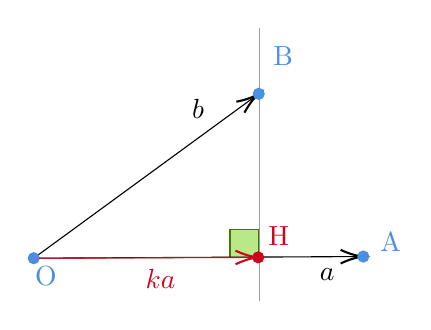
\begin{tikzpicture}[x=0.75pt,y=0.75pt,yscale=-1,xscale=1]
            %Shape: Square [id:dp12053459766383556] 
            \draw  [color={rgb, 255:red, 65; green, 117; blue, 5 }  ,draw opacity=1 ][fill={rgb, 255:red, 184; green, 233; blue, 134 }  ,fill opacity=1 ] (325.15,136.6) -- (338.75,136.6) -- (338.75,150.2) -- (325.15,150.2) -- cycle ;
            %Straight Lines [id:da6437825035131901] 
            \draw [color={rgb, 255:red, 155; green, 155; blue, 155 }  ,draw opacity=1 ]   (339.4,39.8) -- (339.4,171.4) ;
            %Straight Lines [id:da04881680106137909] 
            \draw    (230.6,150.6) -- (337.39,72.58) ;
            \draw [shift={(339,71.4)}, rotate = 143.85] [color={rgb, 255:red, 0; green, 0; blue, 0 }  ][line width=0.75]    (10.93,-3.29) .. controls (6.95,-1.4) and (3.31,-0.3) .. (0,0) .. controls (3.31,0.3) and (6.95,1.4) .. (10.93,3.29)   ;
            %Straight Lines [id:da4755744067309714] 
            \draw    (230.6,150.6) -- (387.4,149.81) ;
            \draw [shift={(389.4,149.8)}, rotate = 179.71] [color={rgb, 255:red, 0; green, 0; blue, 0 }  ][line width=0.75]    (10.93,-3.29) .. controls (6.95,-1.4) and (3.31,-0.3) .. (0,0) .. controls (3.31,0.3) and (6.95,1.4) .. (10.93,3.29)   ;
            %Shape: Circle [id:dp4333439332329939] 
            \draw  [color={rgb, 255:red, 74; green, 144; blue, 226 }  ,draw opacity=1 ][fill={rgb, 255:red, 74; green, 144; blue, 226 }  ,fill opacity=1 ] (336.35,71.4) .. controls (336.35,69.94) and (337.54,68.75) .. (339,68.75) .. controls (340.46,68.75) and (341.65,69.94) .. (341.65,71.4) .. controls (341.65,72.86) and (340.46,74.05) .. (339,74.05) .. controls (337.54,74.05) and (336.35,72.86) .. (336.35,71.4) -- cycle ;
            %Shape: Circle [id:dp18146142560368583] 
            \draw  [color={rgb, 255:red, 74; green, 144; blue, 226 }  ,draw opacity=1 ][fill={rgb, 255:red, 74; green, 144; blue, 226 }  ,fill opacity=1 ] (386.75,149.8) .. controls (386.75,148.34) and (387.94,147.15) .. (389.4,147.15) .. controls (390.86,147.15) and (392.05,148.34) .. (392.05,149.8) .. controls (392.05,151.26) and (390.86,152.45) .. (389.4,152.45) .. controls (387.94,152.45) and (386.75,151.26) .. (386.75,149.8) -- cycle ;
            %Shape: Circle [id:dp6143429578874029] 
            \draw  [color={rgb, 255:red, 74; green, 144; blue, 226 }  ,draw opacity=1 ][fill={rgb, 255:red, 74; green, 144; blue, 226 }  ,fill opacity=1 ] (227.95,150.6) .. controls (227.95,149.14) and (229.14,147.95) .. (230.6,147.95) .. controls (232.06,147.95) and (233.25,149.14) .. (233.25,150.6) .. controls (233.25,152.06) and (232.06,153.25) .. (230.6,153.25) .. controls (229.14,153.25) and (227.95,152.06) .. (227.95,150.6) -- cycle ;
            %Straight Lines [id:da14420862363300013] 
            \draw [color={rgb, 255:red, 208; green, 2; blue, 27 }  ,draw opacity=1 ]   (233.25,150.6) -- (336.75,150.21) ;
            \draw [shift={(338.75,150.2)}, rotate = 179.78] [color={rgb, 255:red, 208; green, 2; blue, 27 }  ,draw opacity=1 ][line width=0.75]    (10.93,-3.29) .. controls (6.95,-1.4) and (3.31,-0.3) .. (0,0) .. controls (3.31,0.3) and (6.95,1.4) .. (10.93,3.29)   ;
            %Shape: Circle [id:dp5627482989492084] 
            \draw  [color={rgb, 255:red, 208; green, 2; blue, 27 }  ,draw opacity=1 ][fill={rgb, 255:red, 208; green, 2; blue, 27 }  ,fill opacity=1 ] (336.1,150.2) .. controls (336.1,148.74) and (337.29,147.55) .. (338.75,147.55) .. controls (340.21,147.55) and (341.4,148.74) .. (341.4,150.2) .. controls (341.4,151.66) and (340.21,152.85) .. (338.75,152.85) .. controls (337.29,152.85) and (336.1,151.66) .. (336.1,150.2) -- cycle ;
            
            % Text Node
            \draw (305.6,73) node [anchor=north west][inner sep=0.75pt]    {$b$};
            % Text Node
            \draw (367.2,154.2) node [anchor=north west][inner sep=0.75pt]    {$a$};
            % Text Node
            \draw (396.4,137.2) node [anchor=north west][inner sep=0.75pt]   [align=left] {\textcolor[rgb]{0.29,0.56,0.89}{A}};
            % Text Node
            \draw (344.8,47.6) node [anchor=north west][inner sep=0.75pt]   [align=left] {\textcolor[rgb]{0.29,0.56,0.89}{B}};
            % Text Node
            \draw (229.95,153.6) node [anchor=north west][inner sep=0.75pt]   [align=left] {\textcolor[rgb]{0.29,0.56,0.89}{O}};
            % Text Node
            \draw (283.2,154.6) node [anchor=north west][inner sep=0.75pt]    {$\textcolor[rgb]{0.82,0.01,0.11}{ka}$};
            % Text Node
            \draw (342.4,134) node [anchor=north west][inner sep=0.75pt]   [align=left] {\textcolor[rgb]{0.82,0.01,0.11}{H}};
        \end{tikzpicture}            
    \end{center}
    \item \textbf{Proiezione punto su retta:} $H = A + \vec{AH} = A + pro(b,a)$, restituisce un punto
    \begin{center}
        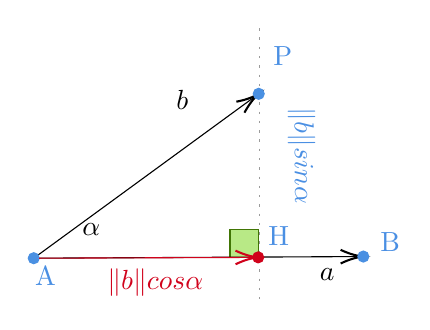
\begin{tikzpicture}[x=0.75pt,y=0.75pt,yscale=-1,xscale=1]
            %Shape: Square [id:dp6295636534815557] 
            \draw  [color={rgb, 255:red, 65; green, 117; blue, 5 }  ,draw opacity=1 ][fill={rgb, 255:red, 184; green, 233; blue, 134 }  ,fill opacity=1 ] (309.15,156.6) -- (322.75,156.6) -- (322.75,170.2) -- (309.15,170.2) -- cycle ;
            %Straight Lines [id:da13541777112119469] 
            \draw [color={rgb, 255:red, 155; green, 155; blue, 155 }  ,draw opacity=1 ] [dash pattern={on 0.84pt off 2.51pt}]  (323.4,59.8) -- (323.4,191.4) ;
            %Straight Lines [id:da2499187369773498] 
            \draw    (214.6,170.6) -- (321.39,92.58) ;
            \draw [shift={(323,91.4)}, rotate = 143.85] [color={rgb, 255:red, 0; green, 0; blue, 0 }  ][line width=0.75]    (10.93,-3.29) .. controls (6.95,-1.4) and (3.31,-0.3) .. (0,0) .. controls (3.31,0.3) and (6.95,1.4) .. (10.93,3.29)   ;
            %Straight Lines [id:da4527457752066615] 
            \draw    (214.6,170.6) -- (371.4,169.81) ;
            \draw [shift={(373.4,169.8)}, rotate = 179.71] [color={rgb, 255:red, 0; green, 0; blue, 0 }  ][line width=0.75]    (10.93,-3.29) .. controls (6.95,-1.4) and (3.31,-0.3) .. (0,0) .. controls (3.31,0.3) and (6.95,1.4) .. (10.93,3.29)   ;
            %Shape: Circle [id:dp6345055124151363] 
            \draw  [color={rgb, 255:red, 74; green, 144; blue, 226 }  ,draw opacity=1 ][fill={rgb, 255:red, 74; green, 144; blue, 226 }  ,fill opacity=1 ] (320.35,91.4) .. controls (320.35,89.94) and (321.54,88.75) .. (323,88.75) .. controls (324.46,88.75) and (325.65,89.94) .. (325.65,91.4) .. controls (325.65,92.86) and (324.46,94.05) .. (323,94.05) .. controls (321.54,94.05) and (320.35,92.86) .. (320.35,91.4) -- cycle ;
            %Shape: Circle [id:dp27313730960245497] 
            \draw  [color={rgb, 255:red, 74; green, 144; blue, 226 }  ,draw opacity=1 ][fill={rgb, 255:red, 74; green, 144; blue, 226 }  ,fill opacity=1 ] (370.75,169.8) .. controls (370.75,168.34) and (371.94,167.15) .. (373.4,167.15) .. controls (374.86,167.15) and (376.05,168.34) .. (376.05,169.8) .. controls (376.05,171.26) and (374.86,172.45) .. (373.4,172.45) .. controls (371.94,172.45) and (370.75,171.26) .. (370.75,169.8) -- cycle ;
            %Shape: Circle [id:dp362138965633202] 
            \draw  [color={rgb, 255:red, 74; green, 144; blue, 226 }  ,draw opacity=1 ][fill={rgb, 255:red, 74; green, 144; blue, 226 }  ,fill opacity=1 ] (211.95,170.6) .. controls (211.95,169.14) and (213.14,167.95) .. (214.6,167.95) .. controls (216.06,167.95) and (217.25,169.14) .. (217.25,170.6) .. controls (217.25,172.06) and (216.06,173.25) .. (214.6,173.25) .. controls (213.14,173.25) and (211.95,172.06) .. (211.95,170.6) -- cycle ;
            %Straight Lines [id:da4483948835610152] 
            \draw [color={rgb, 255:red, 208; green, 2; blue, 27 }  ,draw opacity=1 ]   (217.25,170.6) -- (320.75,170.21) ;
            \draw [shift={(322.75,170.2)}, rotate = 179.78] [color={rgb, 255:red, 208; green, 2; blue, 27 }  ,draw opacity=1 ][line width=0.75]    (10.93,-3.29) .. controls (6.95,-1.4) and (3.31,-0.3) .. (0,0) .. controls (3.31,0.3) and (6.95,1.4) .. (10.93,3.29)   ;
            %Shape: Circle [id:dp6683860916131112] 
            \draw  [color={rgb, 255:red, 208; green, 2; blue, 27 }  ,draw opacity=1 ][fill={rgb, 255:red, 208; green, 2; blue, 27 }  ,fill opacity=1 ] (320.1,170.2) .. controls (320.1,168.74) and (321.29,167.55) .. (322.75,167.55) .. controls (324.21,167.55) and (325.4,168.74) .. (325.4,170.2) .. controls (325.4,171.66) and (324.21,172.85) .. (322.75,172.85) .. controls (321.29,172.85) and (320.1,171.66) .. (320.1,170.2) -- cycle ;
            
            % Text Node
            \draw (282,88.6) node [anchor=north west][inner sep=0.75pt]    {$b$};
            % Text Node
            \draw (351.2,174.2) node [anchor=north west][inner sep=0.75pt]    {$a$};
            % Text Node
            \draw (380.4,157.2) node [anchor=north west][inner sep=0.75pt]   [align=left] {\textcolor[rgb]{0.29,0.56,0.89}{B}};
            % Text Node
            \draw (328.8,67.6) node [anchor=north west][inner sep=0.75pt]   [align=left] {\textcolor[rgb]{0.29,0.56,0.89}{P}};
            % Text Node
            \draw (213.95,173.6) node [anchor=north west][inner sep=0.75pt]   [align=left] {\textcolor[rgb]{0.29,0.56,0.89}{A}};
            % Text Node
            \draw (248.8,174.6) node [anchor=north west][inner sep=0.75pt]    {$\textcolor[rgb]{0.82,0.01,0.11}{\| b\| cos\alpha }$};
            % Text Node
            \draw (326.4,154) node [anchor=north west][inner sep=0.75pt]   [align=left] {\textcolor[rgb]{0.29,0.56,0.89}{H}};
            % Text Node
            \draw (236.8,152.6) node [anchor=north west][inner sep=0.75pt]    {$\alpha $};
            % Text Node
            \draw (351.54,96.66) node [anchor=north west][inner sep=0.75pt]  [rotate=-89.67]  {$\textcolor[rgb]{0.29,0.56,0.89}{\| b\| sin\alpha }$};
        \end{tikzpicture}            
    \end{center}
\end{itemize}

\pagebreak
\subsection{Il prodotto vettoriale}
Il prodotto vettoriale è un operazione che esiste solo in $\mathbb{R}^3$, dati due vettori $\vec{a}$ e $\vec{b}$ tramite il prodotto vettoriale
è possibile definire un vettore $\vec{c}$ ortogonale agli altri due. Di conseguenza se $\vec{a}$ e $\vec{b}$ sono LI si costruisce una base di 
$\mathbb{R}^3$.

Dati due vettori $u = \begin{bmatrix}x_1 \\ x_2 \\ x_3\end{bmatrix}, v=\begin{bmatrix}y_1 \\ y_2 \\ y_3 \end{bmatrix}$, si definisce prodotto vettoriale
tra i due, e si scrive $u\times v$, il vettore
\begin{align*}
    \begin{bmatrix}x_1 \\ x_2 \\ x_3\end{bmatrix} \times \begin{bmatrix}y_1 \\ y_2 \\ y_3 \end{bmatrix}
    = \begin{bmatrix} x_2y_3 - x_3y_2 \\ x_3y_1 - x_1y_3 \\ x_1y_2 - x_2y_1\end{bmatrix}
\end{align*}

\textbf{Nota:} il prodotto vettoriale \underline{non} è commutativo, $e_1 \times e_2 \neq e_2 \times e_1$

Ecco alcune proprietà:
\begin{align*}
    \begin{aligned}
        &\mathbf{e}_1\times\mathbf{e}_2=\mathbf{~e}_3&&\mathbf{e}_2\times\mathbf{e}_1=-\mathbf{e}_3\\
        &\mathbf{e}_2\times\mathbf{e}_3=\mathbf{~e}_1&&\mathbf{e}_3\times\mathbf{e}_2=-\mathbf{e}_1\\
        &\mathbf{e}_3\times\mathbf{e}_1=\mathbf{~e}_2&&\mathbf{e}_1\times\mathbf{e}_3=-\mathbf{e}_2\\ \\
        &\mathbf{e}_1\times\mathbf{e}_1=\mathbf{e}_2\times\mathbf{e}_2=\mathbf{e}_3\times\mathbf{e}_3=\mathbf{0}
    \end{aligned}
\end{align*}

\begin{itemize}
    \item Se $u\times v > 0$ l'orientamento è anti orario
    \item Se $u\times v < 0$ l'orientamento è orario
\end{itemize}

\subsubsection{Teorema}
Se $u,v \in \mathbb{R}^3$ allora
\begin{align*}
    \left\lVert u \times v\right\rVert  = \left\lVert u\right\rVert \left\lVert v\right\rVert sin(\alpha )
\end{align*}

\begin{center}    
    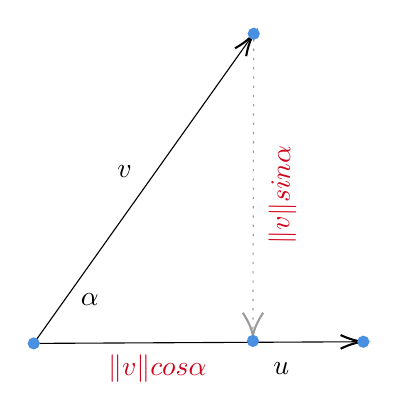
\begin{tikzpicture}[x=0.75pt,y=0.75pt,yscale=-1,xscale=1]
        %Straight Lines [id:da2559707855388087] 
        \draw [color={rgb, 255:red, 155; green, 155; blue, 155 }  ,draw opacity=1 ] [dash pattern={on 0.84pt off 2.51pt}]  (340.6,44.05) -- (340.21,184.75) ;
        \draw [shift={(340.2,186.75)}, rotate = 270.16] [color={rgb, 255:red, 155; green, 155; blue, 155 }  ,draw opacity=1 ][line width=0.75]    (10.93,-4.9) .. controls (6.95,-2.3) and (3.31,-0.67) .. (0,0) .. controls (3.31,0.67) and (6.95,2.3) .. (10.93,4.9)   ;
        %Straight Lines [id:da4779734190453625] 
        \draw    (234.6,190.6) -- (339.44,43.03) ;
        \draw [shift={(340.6,41.4)}, rotate = 125.39] [color={rgb, 255:red, 0; green, 0; blue, 0 }  ][line width=0.75]    (10.93,-3.29) .. controls (6.95,-1.4) and (3.31,-0.3) .. (0,0) .. controls (3.31,0.3) and (6.95,1.4) .. (10.93,3.29)   ;
        %Straight Lines [id:da6234509251246004] 
        \draw    (234.6,190.6) -- (391.4,189.81) ;
        \draw [shift={(393.4,189.8)}, rotate = 179.71] [color={rgb, 255:red, 0; green, 0; blue, 0 }  ][line width=0.75]    (10.93,-3.29) .. controls (6.95,-1.4) and (3.31,-0.3) .. (0,0) .. controls (3.31,0.3) and (6.95,1.4) .. (10.93,3.29)   ;
        %Shape: Circle [id:dp06522483871678564] 
        \draw  [color={rgb, 255:red, 74; green, 144; blue, 226 }  ,draw opacity=1 ][fill={rgb, 255:red, 74; green, 144; blue, 226 }  ,fill opacity=1 ] (337.55,189.4) .. controls (337.55,187.94) and (338.74,186.75) .. (340.2,186.75) .. controls (341.66,186.75) and (342.85,187.94) .. (342.85,189.4) .. controls (342.85,190.86) and (341.66,192.05) .. (340.2,192.05) .. controls (338.74,192.05) and (337.55,190.86) .. (337.55,189.4) -- cycle ;
        %Shape: Circle [id:dp8517909156279818] 
        \draw  [color={rgb, 255:red, 74; green, 144; blue, 226 }  ,draw opacity=1 ][fill={rgb, 255:red, 74; green, 144; blue, 226 }  ,fill opacity=1 ] (390.75,189.8) .. controls (390.75,188.34) and (391.94,187.15) .. (393.4,187.15) .. controls (394.86,187.15) and (396.05,188.34) .. (396.05,189.8) .. controls (396.05,191.26) and (394.86,192.45) .. (393.4,192.45) .. controls (391.94,192.45) and (390.75,191.26) .. (390.75,189.8) -- cycle ;
        %Shape: Circle [id:dp42509862243894725] 
        \draw  [color={rgb, 255:red, 74; green, 144; blue, 226 }  ,draw opacity=1 ][fill={rgb, 255:red, 74; green, 144; blue, 226 }  ,fill opacity=1 ] (231.95,190.6) .. controls (231.95,189.14) and (233.14,187.95) .. (234.6,187.95) .. controls (236.06,187.95) and (237.25,189.14) .. (237.25,190.6) .. controls (237.25,192.06) and (236.06,193.25) .. (234.6,193.25) .. controls (233.14,193.25) and (231.95,192.06) .. (231.95,190.6) -- cycle ;
        %Shape: Circle [id:dp9107538472897923] 
        \draw  [color={rgb, 255:red, 74; green, 144; blue, 226 }  ,draw opacity=1 ][fill={rgb, 255:red, 74; green, 144; blue, 226 }  ,fill opacity=1 ] (337.95,41.4) .. controls (337.95,39.94) and (339.14,38.75) .. (340.6,38.75) .. controls (342.06,38.75) and (343.25,39.94) .. (343.25,41.4) .. controls (343.25,42.86) and (342.06,44.05) .. (340.6,44.05) .. controls (339.14,44.05) and (337.95,42.86) .. (337.95,41.4) -- cycle ;
        
        % Text Node
        \draw (273.6,103.8) node [anchor=north west][inner sep=0.75pt]    {$v$};
        % Text Node
        \draw (348.8,198.6) node [anchor=north west][inner sep=0.75pt]    {$u$};
        % Text Node
        \draw (269.2,194.6) node [anchor=north west][inner sep=0.75pt]    {$\textcolor[rgb]{0.82,0.01,0.11}{\| v\| cos\alpha }$};
        % Text Node
        \draw (256,165.4) node [anchor=north west][inner sep=0.75pt]    {$\alpha $};
        % Text Node
        \draw (346.35,144.21) node [anchor=north west][inner sep=0.75pt]  [rotate=-270.69]  {$\textcolor[rgb]{0.82,0.01,0.11}{\| v\| sin\alpha }$};
    \end{tikzpicture}    
\end{center}

\subsubsection{Area del parallelogramma}
\begin{itemize}
    \item $\left\lVert v\right\rVert sin(\alpha)$ è l'altezza del parallelogramma generato da $u$ e $v$
    \item $\left\lVert u \times v\right\rVert$ è l'area del parallelogramma generato da $u$ e $v$
    \item $\frac{1}{2}\left\lVert u \times v\right\rVert$ è l'area del triangolo generato da $u$ e $v$
\end{itemize}

$$
    sin(\alpha) = \frac{\left\lVert u \times v\right\rVert }{\left\lVert u\right\rVert \left\lVert v\right\rVert }
$$
e quindi
$$
    \alpha = sin^{-1}\left( \frac{\left\lVert u \times v\right\rVert }{\left\lVert u\right\rVert \left\lVert v\right\rVert } \right)
$$

\pagebreak
\subsection{Il prodotto misto}
Il prodotto misto si fa tra 3 vettori e ritorna uno \underline{scalare} (un numero) e non un vettore.
$$
    (a\times b) \cdot c
$$
che è uguale al \textbf{volume} del parallelepipedo generato da $a,b,c$.

\begin{itemize}
    \item $(a\times b) \cdot c > 0\Rightarrow a,b,c$ è una terna destrorsa
    \item $(a\times b) \cdot c < 0\Rightarrow a,b,c$ è una terna sinistrorsa
    \item $(a\times b) \cdot c = 0\Rightarrow a,b,c$ sono linearmente dipendenti
\end{itemize}

\subsubsection{Proprietà}
\begin{align*}
    &\mathbf{a \times b\cdot c}=\mathbf{b\times c\cdot a}=\mathbf{c\times a\cdot b} \\
    &\mathbf{b\times a\cdot c}=\mathbf{c\times b\cdot a}=\mathbf{a\times c\cdot b} \\
    &\mathbf{a\times b\cdot c}=-\mathbf{b\times a\cdot c}
\end{align*}

\begin{align*}
    &k\mathbf{a}\times\mathbf{b}\cdot\mathbf{c}=\mathbf{a}\times k\mathbf{b}\cdot\mathbf{c}=\mathbf{a}\times\mathbf{b}\cdot k\mathbf{c}=k(\mathbf{a}\times\mathbf{b}\cdot\mathbf{c}) \\
    &(ha)\times(jb)\cdot(kc)=(hjk)(a\times b\cdot c)
\end{align*}

\subsubsection{Allineamento di 3 punti}
\begin{itemize}
    \item \textbf{Metodo 1:} i punti $A,B,C$ sono allineati se e solo se $AC = kAB$
    \item \textbf{Metodo 2 (in $\mathbb{R}^3$):} i punti $A,B,C$ sono allineati se e solo se $AB \times AC = 0$
\end{itemize}

\subsubsection{Complanarità di 4 punti}
$$
    (AB \times AC) \cdot AD = 0
$$
se $n = AB \times AC$ dà un vettore ortogonale al piano $ABC$, il punto $D$ invece appartiene a questo piano se e solo se
$AD$ è ortogonale a $n$, ovvero se $n \cdot AD$ è nullo.

\subsubsection{Distanze}
\begin{itemize}
    \item Dal punto $P$ al punto $A$: $\phantom{--}\sqrt{AP \cdot AP}$
    \item Dal punto $P$ alla retta $AB$: $\phantom{--}\frac{\left\lVert AB \times AP\right\rVert }{\left\lVert AB\right\rVert }$
    \begin{center}
        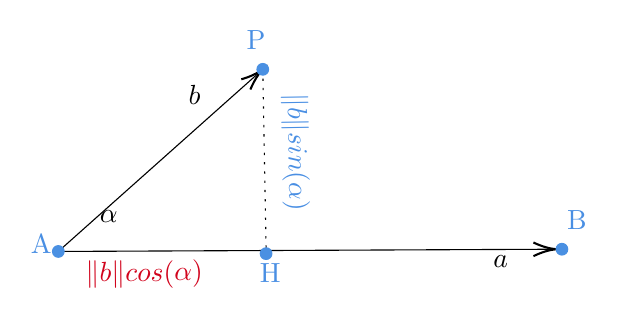
\begin{tikzpicture}[x=0.75pt,y=0.75pt,yscale=-1,xscale=1]
            %Straight Lines [id:da892655129394256] 
            \draw    (210.5,220.75) -- (448.33,219.68) ;
            \draw [shift={(450.33,219.67)}, rotate = 179.74] [color={rgb, 255:red, 0; green, 0; blue, 0 }  ][line width=0.75]    (10.93,-3.29) .. controls (6.95,-1.4) and (3.31,-0.3) .. (0,0) .. controls (3.31,0.3) and (6.95,1.4) .. (10.93,3.29)   ;
            %Straight Lines [id:da6822806692901882] 
            \draw    (210.5,220.75) -- (307.51,134.33) ;
            \draw [shift={(309,133)}, rotate = 138.3] [color={rgb, 255:red, 0; green, 0; blue, 0 }  ][line width=0.75]    (10.93,-3.29) .. controls (6.95,-1.4) and (3.31,-0.3) .. (0,0) .. controls (3.31,0.3) and (6.95,1.4) .. (10.93,3.29)   ;
            %Straight Lines [id:da03778675317968749] 
            \draw  [dash pattern={on 0.84pt off 2.51pt}]  (309,133) -- (310.6,219) ;
            %Shape: Circle [id:dp8171200159632993] 
            \draw  [color={rgb, 255:red, 74; green, 144; blue, 226 }  ,draw opacity=1 ][fill={rgb, 255:red, 74; green, 144; blue, 226 }  ,fill opacity=1 ] (207.7,220.75) .. controls (207.7,219.2) and (208.95,217.95) .. (210.5,217.95) .. controls (212.05,217.95) and (213.3,219.2) .. (213.3,220.75) .. controls (213.3,222.3) and (212.05,223.55) .. (210.5,223.55) .. controls (208.95,223.55) and (207.7,222.3) .. (207.7,220.75) -- cycle ;
            %Shape: Circle [id:dp7640322309786388] 
            \draw  [color={rgb, 255:red, 74; green, 144; blue, 226 }  ,draw opacity=1 ][fill={rgb, 255:red, 74; green, 144; blue, 226 }  ,fill opacity=1 ] (307.8,221.8) .. controls (307.8,220.25) and (309.05,219) .. (310.6,219) .. controls (312.15,219) and (313.4,220.25) .. (313.4,221.8) .. controls (313.4,223.35) and (312.15,224.6) .. (310.6,224.6) .. controls (309.05,224.6) and (307.8,223.35) .. (307.8,221.8) -- cycle ;
            %Shape: Circle [id:dp08802824506738027] 
            \draw  [color={rgb, 255:red, 74; green, 144; blue, 226 }  ,draw opacity=1 ][fill={rgb, 255:red, 74; green, 144; blue, 226 }  ,fill opacity=1 ] (450.33,219.67) .. controls (450.33,218.12) and (451.59,216.87) .. (453.13,216.87) .. controls (454.68,216.87) and (455.93,218.12) .. (455.93,219.67) .. controls (455.93,221.21) and (454.68,222.47) .. (453.13,222.47) .. controls (451.59,222.47) and (450.33,221.21) .. (450.33,219.67) -- cycle ;
            %Shape: Circle [id:dp7912076503628818] 
            \draw  [color={rgb, 255:red, 74; green, 144; blue, 226 }  ,draw opacity=1 ][fill={rgb, 255:red, 74; green, 144; blue, 226 }  ,fill opacity=1 ] (306.2,133) .. controls (306.2,131.45) and (307.45,130.2) .. (309,130.2) .. controls (310.55,130.2) and (311.8,131.45) .. (311.8,133) .. controls (311.8,134.55) and (310.55,135.8) .. (309,135.8) .. controls (307.45,135.8) and (306.2,134.55) .. (306.2,133) -- cycle ;
            
            % Text Node
            \draw (272,139.4) node [anchor=north west][inner sep=0.75pt]    {$b$};
            % Text Node
            \draw (418.8,221.4) node [anchor=north west][inner sep=0.75pt]    {$a$};
            % Text Node
            \draw (196,211.2) node [anchor=north west][inner sep=0.75pt]   [align=left] {\textcolor[rgb]{0.29,0.56,0.89}{A}};
            % Text Node
            \draw (300,113.2) node [anchor=north west][inner sep=0.75pt]   [align=left] {\textcolor[rgb]{0.29,0.56,0.89}{P}};
            % Text Node
            \draw (454.4,200) node [anchor=north west][inner sep=0.75pt]   [align=left] {\textcolor[rgb]{0.29,0.56,0.89}{B}};
            % Text Node
            \draw (306.4,225.2) node [anchor=north west][inner sep=0.75pt]   [align=left] {\textcolor[rgb]{0.29,0.56,0.89}{H}};
            % Text Node
            \draw (229.2,199.8) node [anchor=north west][inner sep=0.75pt]    {$\alpha $};
            % Text Node
            \draw (332.26,143.09) node [anchor=north west][inner sep=0.75pt]  [rotate=-89.05]  {$\textcolor[rgb]{0.29,0.56,0.89}{\| b\| sin( \alpha )}$};
            % Text Node
            \draw (222.35,224.05) node [anchor=north west][inner sep=0.75pt]  [rotate=-359.56]  {$\textcolor[rgb]{0.82,0.01,0.11}{\| b\| cos( \alpha )}$};
        \end{tikzpicture}            
    \end{center}
    \vspace{0.5cm}
    \item Dal punto $P$ al piano $ABC$: $\phantom{--}\frac{\left\lVert AB \times AC \cdot AP\right\rVert }{\left\lVert AB \times AC\right\rVert }$
\end{itemize}

\pagebreak
\subsubsection{Proiezione di un punto su un piano}
\begin{center}
    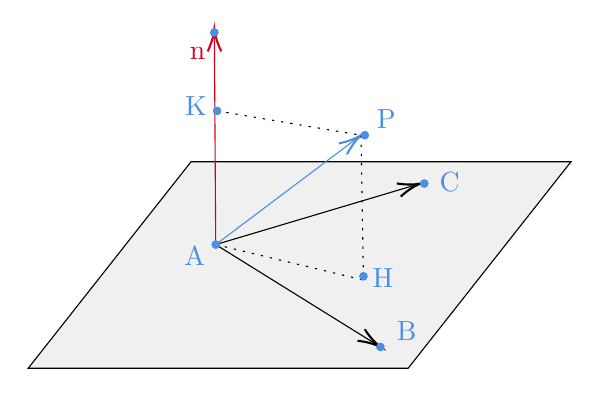
\begin{tikzpicture}[x=0.75pt,y=0.75pt,yscale=-1,xscale=1]
        %Shape: Parallelogram [id:dp9110911154214759] 
        \draw  [fill={rgb, 255:red, 240; green, 240; blue, 240 }  ,fill opacity=1 ] (228.45,151.75) -- (411.5,151.75) -- (333.05,251.25) -- (150,251.25) -- cycle ;
        %Straight Lines [id:da8691855199076285] 
        \draw    (240.33,191.67) -- (317.97,239.94) ;
        \draw [shift={(319.67,241)}, rotate = 211.88] [color={rgb, 255:red, 0; green, 0; blue, 0 }  ][line width=0.75]    (10.93,-3.29) .. controls (6.95,-1.4) and (3.31,-0.3) .. (0,0) .. controls (3.31,0.3) and (6.95,1.4) .. (10.93,3.29)   ;
        %Straight Lines [id:da9679421894754798] 
        \draw    (240.33,191.67) -- (337.08,162.82) ;
        \draw [shift={(339,162.25)}, rotate = 163.4] [color={rgb, 255:red, 0; green, 0; blue, 0 }  ][line width=0.75]    (10.93,-3.29) .. controls (6.95,-1.4) and (3.31,-0.3) .. (0,0) .. controls (3.31,0.3) and (6.95,1.4) .. (10.93,3.29)   ;
        %Straight Lines [id:da8562099048635072] 
        \draw [color={rgb, 255:red, 74; green, 144; blue, 226 }  ,draw opacity=1 ]   (240.33,191.67) -- (308.74,140.2) ;
        \draw [shift={(310.33,139)}, rotate = 143.04] [color={rgb, 255:red, 74; green, 144; blue, 226 }  ,draw opacity=1 ][line width=0.75]    (10.93,-3.29) .. controls (6.95,-1.4) and (3.31,-0.3) .. (0,0) .. controls (3.31,0.3) and (6.95,1.4) .. (10.93,3.29)   ;
        %Straight Lines [id:da1499080300619997] 
        \draw [color={rgb, 255:red, 208; green, 2; blue, 27 }  ,draw opacity=1 ]   (240.33,191.67) -- (239.68,89.67) ;
        \draw [shift={(239.67,87.67)}, rotate = 89.63] [color={rgb, 255:red, 208; green, 2; blue, 27 }  ,draw opacity=1 ][line width=0.75]    (10.93,-3.29) .. controls (6.95,-1.4) and (3.31,-0.3) .. (0,0) .. controls (3.31,0.3) and (6.95,1.4) .. (10.93,3.29)   ;
        %Straight Lines [id:da22301277999575264] 
        \draw  [dash pattern={on 0.84pt off 2.51pt}]  (240.33,191.67) -- (311.5,208.75) ;
        %Straight Lines [id:da0026953899713432206] 
        \draw  [dash pattern={on 0.84pt off 2.51pt}]  (241,127.25) -- (310.33,139) ;
        %Straight Lines [id:da6550164242035883] 
        \draw  [dash pattern={on 0.84pt off 2.51pt}]  (310.33,139) -- (311.5,208.75) ;
        %Shape: Circle [id:dp9257625086160886] 
        \draw  [color={rgb, 255:red, 74; green, 144; blue, 226 }  ,draw opacity=1 ][fill={rgb, 255:red, 74; green, 144; blue, 226 }  ,fill opacity=1 ] (239.19,127.25) .. controls (239.19,126.25) and (240,125.44) .. (241,125.44) .. controls (242,125.44) and (242.81,126.25) .. (242.81,127.25) .. controls (242.81,128.25) and (242,129.06) .. (241,129.06) .. controls (240,129.06) and (239.19,128.25) .. (239.19,127.25) -- cycle ;
        %Shape: Circle [id:dp9845261372187333] 
        \draw  [color={rgb, 255:red, 74; green, 144; blue, 226 }  ,draw opacity=1 ][fill={rgb, 255:red, 74; green, 144; blue, 226 }  ,fill opacity=1 ] (238.52,191.67) .. controls (238.52,190.67) and (239.33,189.85) .. (240.33,189.85) .. controls (241.33,189.85) and (242.15,190.67) .. (242.15,191.67) .. controls (242.15,192.67) and (241.33,193.48) .. (240.33,193.48) .. controls (239.33,193.48) and (238.52,192.67) .. (238.52,191.67) -- cycle ;
        %Shape: Circle [id:dp9890538242111186] 
        \draw  [color={rgb, 255:red, 74; green, 144; blue, 226 }  ,draw opacity=1 ][fill={rgb, 255:red, 74; green, 144; blue, 226 }  ,fill opacity=1 ] (310.33,139) .. controls (310.33,138) and (311.14,137.19) .. (312.15,137.19) .. controls (313.15,137.19) and (313.96,138) .. (313.96,139) .. controls (313.96,140) and (313.15,140.81) .. (312.15,140.81) .. controls (311.14,140.81) and (310.33,140) .. (310.33,139) -- cycle ;
        %Shape: Circle [id:dp2812600709350239] 
        \draw  [color={rgb, 255:red, 74; green, 144; blue, 226 }  ,draw opacity=1 ][fill={rgb, 255:red, 74; green, 144; blue, 226 }  ,fill opacity=1 ] (339,162.25) .. controls (339,161.25) and (339.81,160.44) .. (340.81,160.44) .. controls (341.81,160.44) and (342.63,161.25) .. (342.63,162.25) .. controls (342.63,163.25) and (341.81,164.06) .. (340.81,164.06) .. controls (339.81,164.06) and (339,163.25) .. (339,162.25) -- cycle ;
        %Shape: Circle [id:dp24076253307157125] 
        \draw  [color={rgb, 255:red, 74; green, 144; blue, 226 }  ,draw opacity=1 ][fill={rgb, 255:red, 74; green, 144; blue, 226 }  ,fill opacity=1 ] (309.69,206.94) .. controls (309.69,205.94) and (310.5,205.13) .. (311.5,205.13) .. controls (312.5,205.13) and (313.31,205.94) .. (313.31,206.94) .. controls (313.31,207.94) and (312.5,208.75) .. (311.5,208.75) .. controls (310.5,208.75) and (309.69,207.94) .. (309.69,206.94) -- cycle ;
        %Shape: Circle [id:dp7425254159232946] 
        \draw  [color={rgb, 255:red, 74; green, 144; blue, 226 }  ,draw opacity=1 ][fill={rgb, 255:red, 74; green, 144; blue, 226 }  ,fill opacity=1 ] (317.85,241) .. controls (317.85,240) and (318.67,239.19) .. (319.67,239.19) .. controls (320.67,239.19) and (321.48,240) .. (321.48,241) .. controls (321.48,242) and (320.67,242.81) .. (319.67,242.81) .. controls (318.67,242.81) and (317.85,242) .. (317.85,241) -- cycle ;
        %Shape: Circle [id:dp3954461228898406] 
        \draw  [color={rgb, 255:red, 74; green, 144; blue, 226 }  ,draw opacity=1 ][fill={rgb, 255:red, 74; green, 144; blue, 226 }  ,fill opacity=1 ] (237.85,89.48) .. controls (237.85,88.48) and (238.67,87.67) .. (239.67,87.67) .. controls (240.67,87.67) and (241.48,88.48) .. (241.48,89.48) .. controls (241.48,90.48) and (240.67,91.29) .. (239.67,91.29) .. controls (238.67,91.29) and (237.85,90.48) .. (237.85,89.48) -- cycle ;
        
        % Text Node
        \draw (224,191.33) node [anchor=north west][inner sep=0.75pt]   [align=left] {\textcolor[rgb]{0.29,0.56,0.89}{A}};
        % Text Node
        \draw (326.33,227.67) node [anchor=north west][inner sep=0.75pt]   [align=left] {\textcolor[rgb]{0.29,0.56,0.89}{B}};
        % Text Node
        \draw (347,155.67) node [anchor=north west][inner sep=0.75pt]   [align=left] {\textcolor[rgb]{0.29,0.56,0.89}{C}};
        % Text Node
        \draw (316.67,125.33) node [anchor=north west][inner sep=0.75pt]   [align=left] {\textcolor[rgb]{0.29,0.56,0.89}{P}};
        % Text Node
        \draw (314.67,202) node [anchor=north west][inner sep=0.75pt]   [align=left] {\textcolor[rgb]{0.29,0.56,0.89}{H}};
        % Text Node
        \draw (224.33,119) node [anchor=north west][inner sep=0.75pt]   [align=left] {\textcolor[rgb]{0.29,0.56,0.89}{K}};
        % Text Node
        \draw (226.67,95.33) node [anchor=north west][inner sep=0.75pt]   [align=left] {\textcolor[rgb]{0.82,0.01,0.11}{n}};
    \end{tikzpicture}        
\end{center}

\begin{enumerate}
    \item $n = AB\times AC$
    \item $AK = \text{proiezione di } AP \text{su } n$
    \item $H = P + PH = P + KA$
\end{enumerate}
\textbf{Nota:} possiamo usare qualsiasi vettore parallelo a $n$.


\end{document}